\documentclass{beamer}
% Sans animations
%\documentclass[handout]{beamer}

\usepackage{tikz}
\usepackage{pgfplots}
\tikzstyle{every picture}+=[remember picture]

\setbeamertemplate{footline}[frame number]

\title{ALG2 : recherche d'éléments}
\author{}
\date{loig.jezequel@univ-nantes.fr}

\begin{document}

\frame{
\maketitle
}

\frame{
\frametitle{Tableaux}

\begin{block}{Définition}
Un tableau de taille $n$ est une structure de donnée indicée de 0 à $n-1$ contenant $n$ éléments (tous d'un même type).
\end{block}

\begin{block}{Opérations}
Pour un tableau $t$
\begin{itemize}
  \item $t[i]$ représente l'élément d'indice $i$,
  \item $len(t)$ représente la taille de $t$.
\end{itemize}
\end{block}

\begin{exampleblock}{Exemple}
t = \begin{tabular}{|c|c|c|c|c|}
\hline
12 & 32 & 7 & 23 & 9 \\
\hline
\end{tabular}
\begin{itemize}
  \item les éléments de $t$ sont des entiers,
  \item $len(t) = 5$,
  \item $t[0] = 12$, $t[1] = 32$, $t[2] = 7$, $t[3] = 23$, $t[4] = 9$,
  \item $t[5]$ n'existe pas.
\end{itemize}
\end{exampleblock}
}

\frame{
\frametitle{Les problèmes qu'on se pose}

\vfill

\begin{block}{Problème~: recherche d'élément}
Étant donné un tableau $t$ et un entier $x$, dire si $x$ appartient à $t$ et, si oui, donner un indice $i$ tel que $t[i]=x$.
\end{block}

\vfill

\begin{block}{Problème~: recherche de minimum}
Trouver le plus petit entier dans un tableau $t$, c'est-à-dire trouver un indice $i_{min}$ tel que pour tout $i\in [0,len(t)[$ on a $t[i_{min}]\leq t[i]$.
\end{block}

\vfill

\begin{block}{Problème~: sélection d'éléments}
Étant donné un tableau $t$ et un entier $x$, trouver tous les éléments de $t$ qui sont plus petits que $x$. On veut construire l'ensemble $E$ tel que $y$ appartient à $E$ si et seulement si $y$ appartient à $t$ et $y\leq x$.
\end{block}

\vfill
}

\frame{
\frametitle{Exemples pratiques}

\vfill

\begin{block}{Gestion d'une promotion d'étudiants}
  \begin{itemize}
    \item Savoir si un étudiant appartient à un groupe.
    \item Trouver l'étudiant le plus jeune.
    \item Lister les étudiants qui ont eu la moyenne.
  \end{itemize}
\end{block}

\vfill

\begin{block}{Gestion d'un ensemble de tâches à réaliser}
  \begin{itemize}
    \item Savoir si une tâche a déjà été réalisée.
    \item Trouver la tâche la plus prioritaire.
    \item Lister les tâches qu'il reste à réaliser.
  \end{itemize}
\end{block}

\vfill
}

\frame{
\frametitle{Recherche d'élément}

\begin{block}{Problème}
Étant donné un tableau $t$ et un entier $x$, dire si $x$ appartient à $t$ et, si oui, donner un indice $i$ tel que $t[i]=x$.
\end{block}

\begin{alertblock}{Algorithme}
Soit $i=0$.
Tant que $i<len(t)$, si $t[i] = x$ \tikz[baseline]{\node[fill=red!20, anchor=base, rounded corners=5, draw=red] (retourne) {retourner $(true, i)$};}, sinon augmenter $i$ de 1.
Retourner $(false, -1)$.
\end{alertblock}

\begin{exampleblock}{Exemple}
  \begin{columns}[T]
    \begin{column}{6cm}
      ~~t = \begin{tabular}{|c|c|c|c|c|}
        \hline
        12 & 32 & 7 & 23 & 9 \\
        \hline
      \end{tabular}

      \vspace{0.5cm}

      \begin{itemize}
        \item $x=7$
      \end{itemize}
      \begin{enumerate}
        \item<2-> $t[i] = t[0] = 12 \neq x$, puis $i=1$
        \item<3-> $t[i] = t[1] = 32 \neq x$, puis $i=2$
        \item<4-> $t[i] = t[2] = 7 = x$,\\ retourne $(true, 2)$
      \end{enumerate}
    \end{column}
    \begin{column}{6cm}
      \begin{itemize}
        \item $x=5$
      \end{itemize}
      \begin{enumerate}
        \item<5-> $t[i] = t[0] = 12 \neq x$, puis $i=1$
        \item<6-> $t[i] = t[1] = 32 \neq x$, puis $i=2$
        \item<7-> $t[i] = t[2] = 7 \neq x$, puis $i=3$
        \item<8-> $t[i] = t[3] = 23 \neq x$, puis $i=4$
        \item<9-> $t[i] = t[4] = 9 \neq x$, puis $i=5$
        \item<10> $i \geq len(t)$, retourne $(false, -1)$
      \end{enumerate}
    \end{column}
  \end{columns}
\end{exampleblock}

\begin{tikzpicture}[overlay]
  \node[above right of=retourne, red, yshift=5] (inforet) {termine l'algorithme};
  \path[-, red] (retourne) edge (inforet);
\end{tikzpicture}
}

\frame{
\frametitle{Recherche d'élément~: nombre d'opérations}

\begin{block}{Pourquoi se poser la question du nombre d'opérations ?}
Permet de comparer des algorithmes entre eux, savoir lequel sera le plus efficace en temps de calcul.
\end{block}

\begin{block}{Quelles opérations ?}
Affectations de variables, tests, opérations arithmétiques.
\end{block}

\begin{block}{Remarque}
Pour être vraiment précis il faudrait compter les instructions en langage machine car c'est cela qu'un processeur va exécuter au final.
\begin{itemize}
  \item Dépend du langage, du compilateur, du processeur.
  \item Dépend de l'implantation de l'algorithme.
\end{itemize}
En général on calcule un \alert{ordre de grandeur} du nombre d'opérations en \alert{fonction de la taille de l'entrée}.
\end{block}

}

\frame{
\frametitle{Recherche d'élément~: nombre d'opérations, suite}

\vfill

\begin{block}{Rappel de l'algorithme}
Soit \tikz[baseline]{\node[fill=red!20, anchor=base, rounded corners=5, draw=red] (affectation) {$i=0$};}.
Tant que \tikz[baseline]{\node[fill=red!20, anchor=base, rounded corners=5, draw=red] (test1) {$i<len(t)$};}, si \tikz[baseline]{\node[fill=red!20, anchor=base, rounded corners=5, draw=red] (test2) {$t[i] = x$};} retourner $(true, i)$, sinon \tikz[baseline]{\node[fill=red!20, anchor=base, rounded corners=5, draw=red] (arithmetique) {augmenter $i$};} de 1.
Retourner $(false, -1)$.
\end{block}

\vfill

\begin{block}{Nombre d'opérations}
\begin{itemize}
  \item 1 affectation de variable à l'initialisation.
  \item 2 tests et 1 opération arithmétique par tour de boucle.
\end{itemize}
Soit $3k + 1$ opérations, où $k$ est le nombre de tours de boucle.
\end{block}

\vfill

\begin{block}{Nombre d'opérations dans le pire cas}
On ne peut pas savoir à l'avance le nombre de tours de boucle effectués, on considère ce qui va se passer au pire~: $k=len(t)$.
\end{block}

\vfill

\begin{tikzpicture}[overlay]
  \node[above right of=test1, red, yshift=5] (test) {tests};
  \path[-, red] (test) edge (test1);
  \path[-, red] (test) edge (test2);
  \node[below right of=arithmetique, red, xshift=50] (opar) {opération arithmétique};
  \path[-, red] (opar.west) edge (arithmetique);
  \node[above right of=affectation, red, yshift=10] (aff) {affectation de variable};
  \path[-, red] (aff) edge (affectation);
\end{tikzpicture}
}

\frame{
\frametitle{Recherche de minimum}

\begin{block}{Problème}
Trouver le plus petit entier dans un tableau $t$, c'est-à-dire trouver un indice $i_{min}$ tel que pour tout $i\in [0,len(t)[$ on a $t[i_{min}]\leq t[i]$.
\end{block}

\begin{alertblock}{Algorithme}
Soit $i=1$ et soit $i_{min} = 0$.
Tant que $i<len(t)$, si $t[i] < t[i_{min}]$ poser $i_{min} = i$, dans tous les cas augmenter $i$ de 1.
Retourner $i_{min}$.
\end{alertblock}

\begin{exampleblock}{Exemple}
t = \begin{tabular}{|c|c|c|c|c|}
\hline
12 & 32 & 7 & 23 & 9 \\
\hline
\end{tabular}
\begin{enumerate}
  \item<2-> $t[i] = t[1] > t[0] = t[i_{min}]$, $i_{min}$ ne change pas, puis $i=2$,
  \item<3-> $t[i] = t[2] < t[0] = t[i_{min}]$, donc $i_{min} = 2$, puis $i = 3$,
  \item<4-> $t[i] = t[3] >t[2] = t[i_{min}]$, $i_{min}$ ne change pas, puis $i=4$,
  \item<5-> $t[i] = t[4] > t[2] = t[i_{min}]$, $i_{min}$ ne change pas, puis $i=5$,
  \item<6> $i = 5 = len(t)$, on retourne $i_{min} = 2$.
\end{enumerate}
\end{exampleblock}
}

\frame{
\frametitle{Recherche de minimum~: nombre d'opérations}

\begin{block}{Rappel de l'algorithme}
Soit \tikz[baseline]{\node[fill=red!20, anchor=base, rounded corners=5, draw=red] (affectation1) {$i=1$};} et soit \tikz[baseline]{\node[fill=red!20, anchor=base, rounded corners=5, draw=red] (affectation2) {$i_{min} = 0$};}.
Tant que \tikz[baseline]{\node[fill=red!20, anchor=base, rounded corners=5, draw=red] (test1) {$i<len(t)$};}, si \tikz[baseline]{\node[fill=red!20, anchor=base, rounded corners=5, draw=red] (test2) {$t[i] < t[i_{min}]$};} poser \tikz[baseline]{\node[fill=red!20, anchor=base, rounded corners=5, draw=red] (affectation3) {$i_{min} = i$};}, dans tous les cas \tikz[baseline]{\node[fill=red!20, anchor=base, rounded corners=5, draw=red] (arithmetique) {augmenter $i$};} de 1.
Retourner $i_{min}$.
\end{block}

\begin{block}{Nombre d'opérations}
\begin{itemize}
\item 2 opérations à l'initialisation.
\item 3 opérations à chaque tour de boucle.
\item 1 opération par tour de boucle où la conditionnelle a lieu.
\end{itemize}
Soit $3\times{}(len(t)-1) + k + 2$ opérations, avec $k$ le nombre de tours de boucle où la conditionnelle a lieu.
\end{block}

\begin{block}{Nombre d'opérations dans le pire cas}
La conditionnelle a lieu tout le temps~: $k = (len(t)-1)$
\end{block}

}

\frame{
\frametitle{Sélection d'éléments}

\begin{block}{Problème}
Étant donné un tableau $t$ et un entier $x$, trouver tous les éléments de $t$ qui sont plus petits que $x$. On veut construire l'ensemble $E$ tel que $y$ appartient à $E$ si et seulement si $y$ appartient à $t$ et $y\leq x$.
\end{block}

\begin{alertblock}{Algorithme}
  Soit $i=0$ et soit $E = \emptyset$.
  Tant que $i<len(t)$, si $t[i] \leq x$ ajouter $t[i]$ dans $E$, dans tous les cas augmenter $i$ de 1.
  Retourner $E$.
\end{alertblock}

\begin{exampleblock}{Exemple}
t = \begin{tabular}{|c|c|c|c|c|}
\hline
12 & 32 & 7 & 23 & 9 \\
\hline
\end{tabular}
et $x = 10$
\begin{enumerate}
  \item<2-> $t[i] = t[0] > 10$, $E$ ne change pas, puis $i=1$,
  \item<3-> $t[i] = t[1] > 10$, $E$ ne change pas, puis $i = 2$,
  \item<4-> $t[i] = t[2] \leq 10$, $E = \{7\}$, puis $i=3$,
  \item<5-> $t[i] = t[3] > 10$, $E$ ne change pas, puis $i=4$,
  \item<6-> $t[i] = t[4] \leq 10$, $E = \{7, 9\}$, puis $i=5$,
  \item<7> $i = 5 = len(t)$, on retourne $E = \{7, 9\}$.
\end{enumerate}
\end{exampleblock}
}

\frame{
\frametitle{Sélection d'éléments~: nombre d'opérations}

\vfill

\begin{block}{Rappel de l'algorithme}
  Soit $i=0$ et soit \tikz[baseline]{\node[fill=red!20, anchor=base, rounded corners=5, draw=red] (affectation1) {$E = \emptyset$};}.
  Tant que $i<len(t)$, si $t[i] \leq x$ \tikz[baseline]{\node[fill=red!20, anchor=base, rounded corners=5, draw=red] (affectation2) {ajouter $t[i]$ dans $E$};}, dans tous les cas augmenter $i$ de 1.
  Retourner $E$.
\end{block}

\vfill

\begin{block}{Nombre d'opérations et nombre d'opérations dans le pire cas}
Similaires à la recherche de minimum à condition que les opérations sur les ensemble soient simples.
\end{block}

\vfill

\begin{tikzpicture}[overlay]
  \node[above right of=affectation1, red, xshift=40, yshift=5] (aff1) {affectation ?};
  \path[-, red] (affectation1) edge (aff1);
  \node[below right of=affectation2, red, xshift=40, yshift=-5] (aff2) {affectation ?};
  \path[-, red] (affectation2) edge (aff2);
\end{tikzpicture}
}

\frame{
\frametitle{Peut-on faire mieux ?}

\begin{block}{Bilan des nombres d'opérations nécessaires}
\begin{description}
\item[Recherche d'élément.] $3\times len(t) + 1$
\item[Recherche de minimum et sélection d'éléments.] $4\times len(t) - 2$
\end{description}
\end{block}

\begin{block}{Ordres de grandeur}
Les constantes peuvent varier dans ces nombres d'opérations (en fonction de l'implantation de l'algorithme, du compilateur, du processeur) mais ils restent linéaires en la taille du tableau.
\end{block}

\begin{block}{Des algorithmes pour réduire l'ordre de grandeur}
On ne peut pas faire mieux sur des tableaux quelconques, mais si on sait que les tableaux qu'on aura en entrée ont certaines propriétés c'est différent~:
\begin{itemize}
\item borne sur la valeur maximum qu'ils contiennent,
\item \alert{valeurs triées},
\item etc
\end{itemize}
\end{block}

}

\frame{
\frametitle{Recherche d'élément dans un tableau trié}

\begin{block}{Tableau trié}
Étant donnés un tableau $t$ et un ordre total $\leq$ sur les éléments du tableau, on dit que $t$ est un tableau trié si et seulement si $\forall i < j \in [0, len(t)[, t[i]\leq t[j]$.
\end{block}

\begin{block}{Remarque}
Dans ce cours on utilise des tableaux d'entiers, et on prendra la relation \emph{plus petit ou égal} pour les trier.
\end{block}

\begin{exampleblock}{Recherche efficace dans un tableau trié}
  t = \only<1>{\begin{tabular}{|c|c|c|c|c|c|c|}
  \hline
  12 & 32 & 7 & 23 & 9 & 11 & 29 \\
  \hline
\end{tabular}}\only<2->{\begin{tabular}{|c|c|c|c|c|c|c|}
\hline
7 & 9 & 11 & 12 & 23 & 29 & 32 \\
\hline
\end{tabular}}
\begin{itemize}
\item<2-> Comment trouver un élément en regardant strictement moins de 7 cases ? (pire cas de l'algorithme vu précédemment)
\item<3-> Recherche dichotomique~: exemple pour $x=11$
\begin{enumerate}
\item<4-> indices $[0,7[$, le milieu est $3$ et $t[3] = 12>x$, $x$ ne peut être trouvé que dans les indices $[0,2]$,
\item<5-> indices $[0,3[$, le milieu est $1$ et $t[1] = 9 < x$, $x$ ne peut être trouvé qu'à l'indice $2$,
\item<6> $t[2] = 11 = x$, on a trouvé.
\end{enumerate}
\end{itemize}
\end{exampleblock}

}

\frame{
\frametitle{Recherche dichotomique d'élément dans un tableau trié}

\begin{alertblock}{Algorithme, recherche dichotomique de $x$ dans $t$ trié}
Soit $debut=0$, soit $fin=len(t)$.\\
Tant que $debut<fin$,\\
~~~~ soit $milieu=(debut+fin)/2$,\\
~~~~ si $t[milieu] = x$, retourner $(true, milieu)$,\\
~~~~ sinon si $t[milieu]>x$, poser $fin=milieu$,\\
~~~~ sinon (si $t[milieu]<x$), poser $debut=milieu+1$.\\
Retourner $(false, -1)$.
\end{alertblock}

\begin{exampleblock}{Exemple}
  \begin{tabular}{|c|c|c|c|c|c|c|}
  \hline
  7 & 9 & 11 & 12 & 23 & 29 & 32 \\
  \hline
  \end{tabular}
  on recherche $x=11$.
  \begin{enumerate}
    \item<2-> $milieu = (0 + 7)/2 = 3$, $t[3]=12>x$, donc $debut$ ne change pas et $fin = 3$.
    \item<3-> $milieu = (0 + 3)/2 = 1$, $t[1]=9<x$, donc $debut=1+1=2$ et $fin$ ne change pas.
    \item<4> $milieu = (2 + 3)/2 = 2$, $t[2]=11=x$, donc on retourne $(true, 2)$.
  \end{enumerate}
\end{exampleblock}
}

\frame{
\frametitle{Recherche dichotomique~: nombre d'opérations}

\begin{block}{Rappel de l'algorithme}
Soit \tikz[baseline]{\node[fill=red!20, anchor=base, rounded corners=5, draw=red] (affectation1) {$debut=0$};}, soit \tikz[baseline]{\node[fill=red!20, anchor=base, rounded corners=5, draw=red] (affectation2) {$fin=len(t)$};}.\\
Tant que \tikz[baseline]{\node[fill=red!20, anchor=base, rounded corners=5, draw=red] (test1) {$debut<fin$};},\\
~~~~ soit \tikz[baseline]{\node[fill=red!20, anchor=base, rounded corners=5, draw=red] (arithmetique1) {$milieu=(debut+fin)/2$};},\\
~~~~ si \tikz[baseline]{\node[fill=red!20, anchor=base, rounded corners=5, draw=red] (test2) {$t[milieu] = x$};}, retourner $(true, milieu)$,\\
~~~~ sinon si \tikz[baseline]{\node[fill=red!20, anchor=base, rounded corners=5, draw=red] (test3) {$t[milieu]<x$};}, poser \tikz[baseline]{\node[fill=red!20, anchor=base, rounded corners=5, draw=red] (affectation3) {$fin=milieu$};},\\
~~~~ sinon (si $t[milieu]>x$), poser \tikz[baseline]{\node[fill=red!20, anchor=base, rounded corners=5, draw=red, dashed] (affectation4) {$debut=milieu+1$};}.\\
Retourner $(false, -1)$.
\end{block}

\begin{block}{Nombre d'opérations dans le pire cas}
$5\times k + 2$ où $k$ est le nombre de tours de boucle dans le pire cas.
\end{block}

\begin{block}{Tours de boucle dans le pire cas}
À chaque tour on divise par 2 la taille de l'intervalle $[debut, fin[$ et sa taille initiale est $len(t)$. Donc on fait $\log_2(len(t))$ tours.
\end{block}

\begin{tikzpicture}[overlay]
  \node[right of=affectation3, red, xshift=70, yshift=10] (uneseule) {pas au même tour};
  \path[-, red] (uneseule) edge (affectation3);
  \path[-, red] (uneseule) edge (affectation4);
\end{tikzpicture}
}

\frame{
\frametitle{Recherche dichotomique/séquentielle dans un tableau trié}

\begin{center}
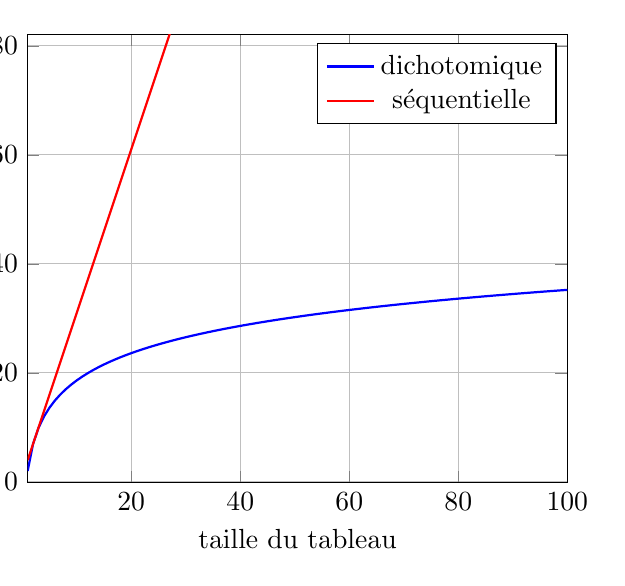
\begin{tikzpicture}[trim axis left]
\begin{axis}[domain=1:100,
  samples=100,
  enlarge x limits=false,
  grid=both,
  no markers,
  axis equal,
  ymin=0., ymax=82.,
  xmin=1., xmax=100.,
  xlabel={taille du tableau},
  ylabel={nombre d'opérations}]
\addplot +[thick] {5*ln(x)/ln(2)+2};
\addlegendentry{dichotomique}
\addplot +[thick] {3*x+1};
\addlegendentry{séquentielle}
\end{axis}
\end{tikzpicture}
\end{center}
}

\frame{
\frametitle{Remarques finales}

\begin{block}{Recherche de minimum dans un tableau trié}
Simplement prendre la valeur de la première case du tableau.
\end{block}

\begin{block}{Sélection d'éléments dans un tableau trié}
Chercher le plus grand élément à sélectionner par dichotomie, puis prendre tous ceux qui sont avant lui dans le tableau.
\end{block}

\begin{block}{Trier un tableau}
  Pour vraiment comparer le nombre d'opérations nécessaires à la recherche séquentielle et à la recherche dichotomique, il faut prendre en compte le tri du tableau~:
  \begin{itemize}
    \item pour chercher une fois un élément ce n'est pas rentable de trier,
    \item si on doit très souvent chercher des éléments ça devient rentable.
  \end{itemize}
  Les algorithmes de tri seront le sujet d'un prochain cours.
\end{block}

}

% preuves de correction des algorithmes

\end{document}
